\StartPlate{V02}{One candidate must satisfy both conditions}{Separate existential statements cannot be joined by changing the witness.}
\begin{center}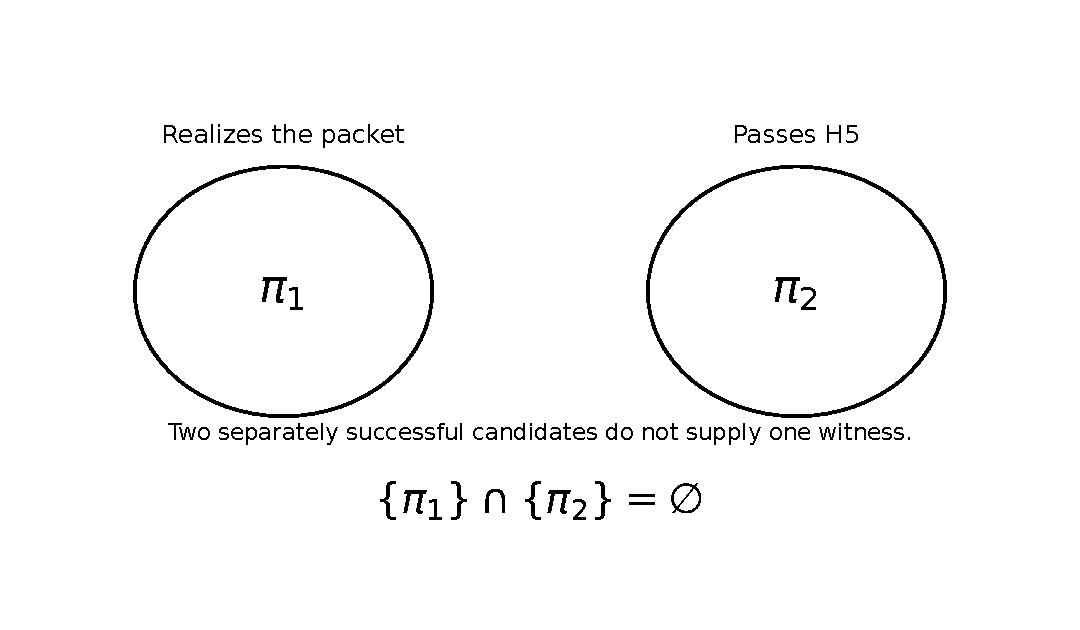
\includegraphics[width=\linewidth]{figures/V02.pdf}\end{center}
Let $A=\{\pi:R(d,\pi)\}$ and $B=\{\pi:H5(\pi)\}$. The desired comparison uses a member of $A\cap B$. The diagram is an exact two-element countermodel: $A=\{\pi_1\}$ and $B=\{\pi_2\}$, with $\pi_1\ne\pi_2$. Each condition has a witness. Their conjunction has none.
\[
(\exists\pi\,R(d,\pi))\land(\exists\pi\,H5(\pi))
\quad\not\Rightarrow\quad
\exists\pi\,(R(d,\pi)\land H5(\pi)).
\]
There is a second pitfall. An implication about every realizer can be true when there are no realizers. A comparison interface whose structure already contains an existence field does not construct that field merely by using it.

These finite sets are logical illustrations, not a claim that the arithmetic realization and H5 classes are actually disjoint. Their purpose is to make a change of candidate visible before it enters a proof.
\vfill\PlateSource{Exact logical countermodel}{Part I, Section 1.2}{6}
